\documentclass[13pt,aspectratio=169,t,xcolor=table]{beamer}
\usepackage[utf8]{inputenc}

\usepackage{booktabs} 
\usepackage{subcaption}
\usepackage{adjustbox}
\usepackage{adjustbox}

\usetheme{Ufg}

%-------------------------------------theorems--------------
\newtheorem{conj}{Conjetura}
\newtheorem{defi}{Definição}
\newtheorem{teo}{Teorema}
\newtheorem{lema}{Lema}
\newtheorem{prop}{Proposição}
\newtheorem{cor}{Corolário}
\newtheorem{ex}{Exemplo}
\newtheorem{exer}{Exercício}

\setbeamertemplate{theorems}[numbered]
\setbeamertemplate{caption}[numbered]

%-------------------------------------------------------------%
%----------------------- Primary Definitions -----------------%

% This command set the default Color, is also possible to choose a custom color
\setPrimaryColor{TorVergataGreen} 

% First one is logo in title slide (we recommend use a horizontal image), and second one is the logo used in the remaining slides (we recommend use a square image)
\setLogos{lib/logos/LOGO-ATENEO_BIANCO_20230308.png}{lib/logos/LOGO-ATENEO_Variante1_Bianco_20230307.png} 


% -------------------------------------- Title Slide Information
\begin{document}
\title[Inf UFG]{Hard Disk Failure Data Processing}
\subtitle{Corso di Sistemi ed Architetture per Big Data}

\author{
    \begin{tabular}{c c}
    Luca Falasca & Matteo Conti \\
    0334722 & 0323728
  \end{tabular}
}

\institute[UFG] % (optional)
{
  Progetto 1 - Stream processing
}
\date{2024}
%-----------------------The next statement creates the title page.
\frame[noframenumbering]{\titlepage}


%------------------------------------------------Slide 1
\setLayout{vertical} % This command define the layout. 'vertical' can be replace with 'horizontal', 'blank, 'mainpoint', 'titlepage'

\begin{frame}
    \frametitle{Indice}
    \tableofcontents
\end{frame}
%---------------------------------------------------------

%---------------------INTRODUZIONE---------------------------
\section{Introduzione}
%---------------------------------------------------------Slide 2
\setLayout{mainpoint}
\setBGColor{TorVergataGreen}
\begin{frame}{}
    \frametitle{Introduzione}
\end{frame}
%---------------------------------------------------------

\subsection{Obbiettivi}
%---------------------------------------------------------Slide 3
\setLayout{vertical}
\begin{frame}{Obbiettivi}
    Il progetto verte sull'analisi di un dataset contenente dati riguardanti il monitoraggio di dischi rigidi installati all'interno di un cluster di server gestito da un cloud provider, in particolare si vuole: 
    \vspace{0.3cm}
    \begin{itemize}
        \item Simulare l'invio in real time dei dati
        \item Realizzare una pipeline di elaborazione real time dei dati
        \item Eseguire le query richieste dalla specifica
        \item Analizzare le performance ottenute
    \end{itemize}
    \vspace{0.3cm}
    \begin{figure}
        \raggedright
        \hspace{2cm}
        
\includegraphics[width=.7\textwidth]{res/intro_icon.png}
    \end{figure}
\end{frame}
%---------------------------------------------------------

%---------------------------------------------------------Slide 4
\subsection{Dataset}
\setLayout{vertical}
\begin{frame}{Dataset}
    Il dataset fornito è una versione ridotta di quello presentato nel Grand Challenge della conferenza ACM DEBS 2024. Delle numerose colonne presenti nel dataset, ne verranno selezionate
    solamente sette, in particolare:
    \begin{itemize}
        \item \textit{date}: data della misurazione nel formato 'YYYY-MM-DD'
        \item \textit{serial\_number}: identificativo del disco rigido
        \item \textit{model}: modello del disco rigido
        \item \textit{s9\_power\_on\_hours}: tempo di accensione del disco rigido in ore
        \item \textit{s194\_temperature\_celsius}: temperatura del disco rigido in gradi Celsius
        \item \textit{vault\_id}: identificativo del gruppo di storage server a cui il disco rigido appartiene
        \item \textit{failure}: flag che indica se il disco rigido ha subito una failure o meno
    \end{itemize}
\end{frame}
%---------------------------------------------------------

%---------------------PIPELINE---------------------------
\section{Pipeline}
%---------------------------------------------------------Slide 5
\setLayout{mainpoint}
\setBGColor{TorVergataGreen}
\begin{frame}{}
    \frametitle{Pipeline}
\end{frame}
%---------------------------------------------------------

%---------------------------------------------------------Slide 6
\setLayout{vertical}
\begin{frame}{Pipeline}
    La pipeline di elaborazione dati è stata containerizzata e deployata tramite docker compose ed è composta da tre componenti:
    \begin{itemize}
        \item Data ingestion
        \item Data processing
        \item Data output
    \end{itemize}
    \begin{adjustbox}{margin=0cm 0cm 0cm 0.9cm, center}% left, bottom, right, top
        
\includegraphics[width=.9\textwidth]{res/pipeline.png}
    \end{adjustbox}
\end{frame}
%---------------------------------------------------------

\subsection{Data ingestion}
\begin{frame}{Data ingestion}
    \begin{itemize}
        \item \textbf{Replay Accelerato del Dataset}
            \begin{itemize}
                \item Fattore di accelerazione: 3600 (1 secondo reale = 1 ora simulata)
            \end{itemize}
        \item \textbf{Granularità Giornaliera}
            \begin{itemize}
                \item Dati giornalieri spalmati uniformemente
                \item Divisione logica della giornata in 150000 parti
                \item Ogni parte rappresenta 1/150000 di giorno
            \end{itemize}
        \item \textbf{Invio delle Tuple}
            \begin{itemize}
                \item Calcolo del tempo di invio della prima tupla
                \item Sleep per riempire lo slot residuo dopo l'invio di ogni tupla
                \item Sleep finale per riempire il tempo rimanente alla fine della giornata
            \end{itemize}
        \item \textbf{Pubblicazione su Kafka}
            \begin{itemize}
                \item Dati pubblicati su un topic dedicato
                \item Consumo dei dati tramite Flink
            \end{itemize}
    \end{itemize}
\end{frame}

\subsection{Data processing}
\begin{frame}{Data rocessing}
Per il processamento streaming è stato utilizzato il framework Apache Flink, con un cluster formato da un job manager ed task manager dotato di un solo task slot, tali valori sono configurabili.
\begin{adjustbox}{margin=0cm 0cm 0cm 1cm, center}% left, bottom, right, top
    
\includegraphics[width=.5\textwidth]{res/flink_icon.png}
\end{adjustbox}
\end{frame}

\begin{frame}{Data Processing-Query 1 (1)}
    \textbf{Q1:} Per i vault con identificativo compreso tra 1000 e 1020, calcolare il numero di
    eventi, il valor medio e la deviazione standard della temperatura misurata sui suoi hard disk utilizzando un algoritmo per il calcolo online di tali statistiche. La query va eseguita con finestre di 1 giorno, 3 giorni e globale.
    \begin{adjustbox}{margin=0cm 0cm 0cm 1cm, center}% left, bottom, right, top
        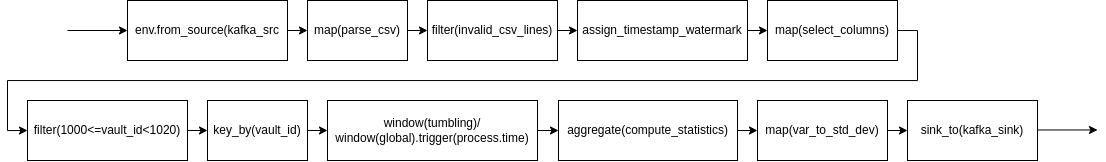
\includegraphics[width=1\textwidth]{res/query1_dag.png}
    \end{adjustbox}
\end{frame}
\begin{frame}{Data Processing-Query 1 (2)}
    \textbf{Calcolo media e deviazione standard:}
    Per il calcolo online della media e della deviazione standard è stato utilizzato l'algoritmo di Wellford in particolare, tali statistiche sono calcolate nell'aggreagate come:
    \begin{equation}
        \begin{aligned}
            \overline{x}_{k+1} &= \overline{x}_k + \frac{x_{k+1} - \overline{x}_k}{k+1} \\
            \sigma^2_{k+1} &= \sigma^2_k + \frac{(x_{k+1} - \overline{x}_k)(x_{k+1} - \overline{x}_{k+1})}{k+1}
        \end{aligned}
    \end{equation}
    Come si può vedere in realtà viene calcolata la varianza, successivamente verrà calcolata la deviazione standard come $\sigma = \sqrt{\sigma^2}$
\end{frame}

\begin{frame}{Data Processing-Query 2}
    \textbf{Q2:} 
    Calcolare la classifica aggiornata in tempo reale dei 10 vault che registrano il pi`u alto numero di falli-
    menti nella stessa giornata. Per ogni vault, riportare il numero di fallimenti ed il modello e numero
    seriale degli hard disk guasti. La query va eseguita con finestre di 1 giorno, 3 giorni e globale.
    \begin{adjustbox}{margin=0cm 0cm 0cm 1cm, center}% left, bottom, right, top
        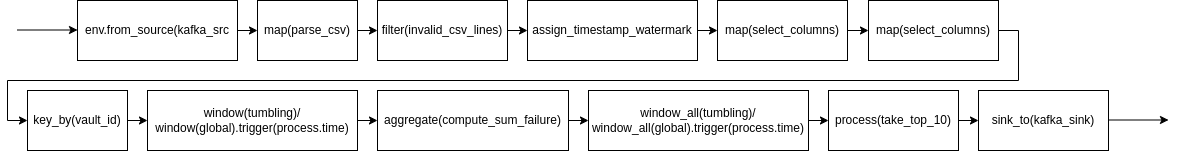
\includegraphics[width=1\textwidth]{res/query2_dag.png}
    \end{adjustbox}
\end{frame}

\begin{frame}{Data Processing-Query 3 (1)}
    \textbf{Q3:} Calcolare il minimo, 25-esimo, 50-esimo, 75-esimo percentile e massimo delle ore di funzionamento
    degli hark disk per i vault con identificativo tra 1090 e 1120, senza accumulare i valori per eseguire il calcolo. La query va eseguita con finestre di 1 giorno, 3 giorni e globale.
    \begin{adjustbox}{margin=0cm 0cm 0cm 1cm, center}% left, bottom, right, top
        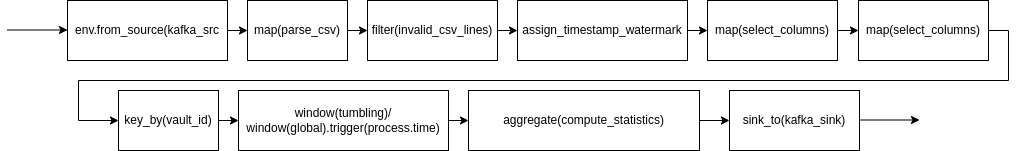
\includegraphics[width=1\textwidth]{res/query3_dag.png}
    \end{adjustbox}
\end{frame}

\begin{frame}{Data Processing-Query 3 (2)}
    \textbf{Calcolo percentili:} 
    Per il calcolo dei percentili è stato utilizzato il PSquare il quale è un algoritmo che permette di calcolare un approssimazione di tali statistiche senza salvare le osservazioni.\\
    \vspace{1cm}
    \textbf{Calcolo minimo e massimo:} 
    Per quanto riguarda minimo e massimo dato l'aggregatore osserva tutte le tuple si è scelto di non approssimarli ma di effettuarne un calcolo esatto confrontando il valore del campo \textit{s9\_power\_on\_hours} della nuova tupla con il valore attuale presente nell'accumulator dell'aggregatore.
\end{frame}

\subsection{Data Output}
\begin{frame}{Data Output}
Per la scrittura dell'output del processamento è stato utilizzato Apache Kafka, in particolare sono stati creati tre topic, uno per ogni query, in cui vengono scritti i risultati delle stesse. I topic sono stati creati tramite un'apposita API di Kafka e vengono consumati da un'applicazione esterna che si occupa di scrivere i risultati su file in formato CSV.
\begin{adjustbox}{margin=0cm 0cm 0cm 1cm, center}% left, bottom, right, top
    
\includegraphics[width=0.8\textwidth]{res/output.png}
\end{adjustbox}
\end{frame}


%---------------------CONCLUSIONI---------------------------
\section{Conclusioni}
\setLayout{mainpoint}
\setBGColor{TorVergataGreen}
\begin{frame}{}
    \frametitle{Conclusioni}
\end{frame}

\setLayout{vertical}
\subsection{Risultati}

\subsection{Performance}
\begin{frame}
    \frametitle{Metriche per le Query}
    \begin{itemize}
        \item \textbf{Latenza}
            \begin{itemize}
                \item Utilizzo di una metrica custom con l'oggetto \texttt{Gauge} offerto da Flink
                \item Fornisce metriche on demand
            \end{itemize}
        \item \textbf{Throughput}
            \begin{itemize}
                \item Utilizzo della metrica built-in di Flink \texttt{NumRecordsOutPerSecond}
                \item Misura il throughput in elementi al secondo
            \end{itemize}
    \end{itemize}
    \vspace{0.5cm}
    \begin{itemize}
        \item Entrambe le metriche sono disponibili tramite l'interfaccia web di Flink
        \item Accessibili tramite REST API
    \end{itemize}
    \vspace{0.5cm}
    \begin{itemize}
        \item Campionamento delle metriche ad intervalli regolari di 1 secondo
        \item Utilizzo di uno script Python per richiedere le metriche al job manager via REST API
        \item Salvataggio dei risultati in un file CSV per la successiva visualizzazione grafica
    \end{itemize}
\end{frame}

\begin{frame}{}
    \frametitle{Query1}
    \begin{columns}
        \column{0.5\textwidth}
        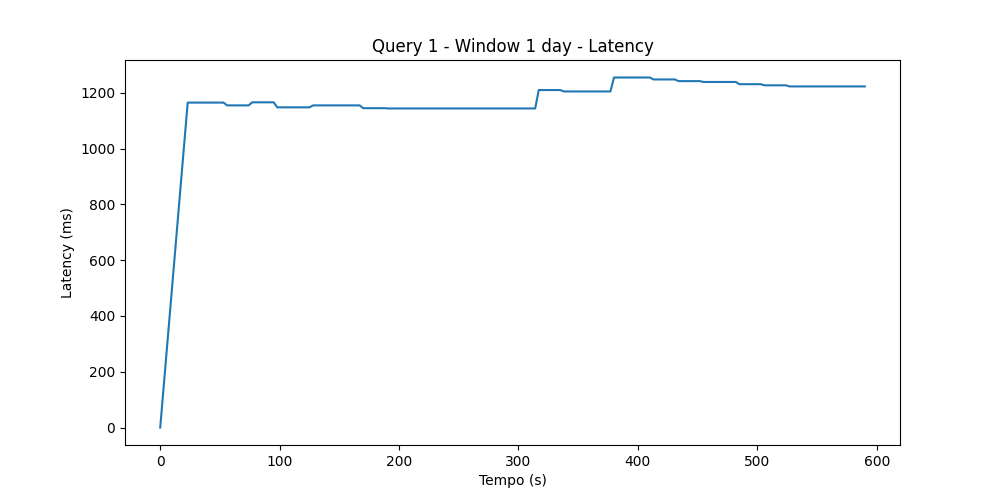
\includegraphics[width=.7\textwidth]{res/q1_w1_latency.png}
        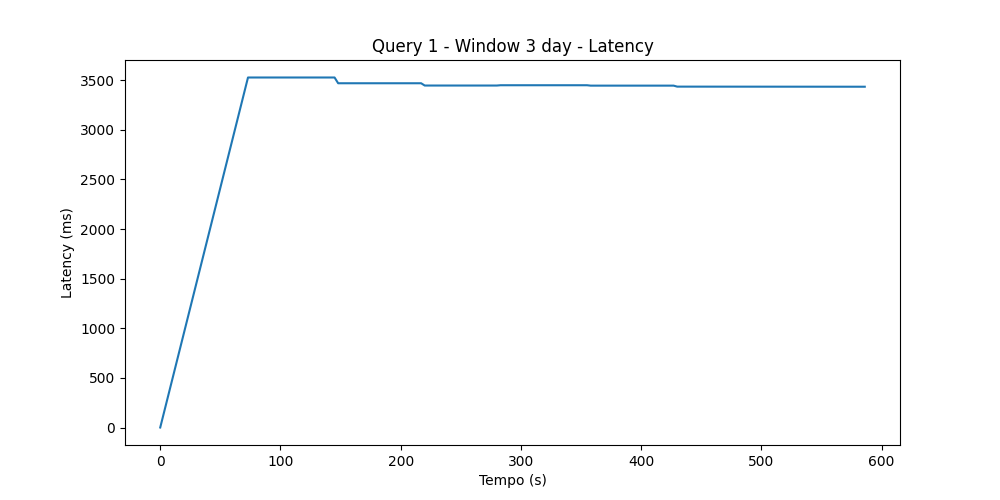
\includegraphics[width=.7\textwidth]{res/q1_w2_latency.png}
        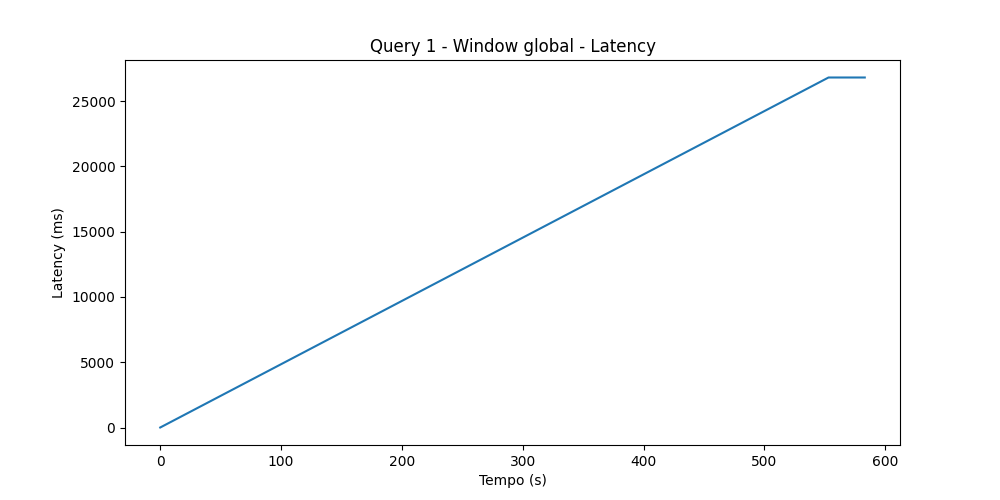
\includegraphics[width=.7\textwidth]{res/q1_w3_latency.png}
        \column{0.5\textwidth}
        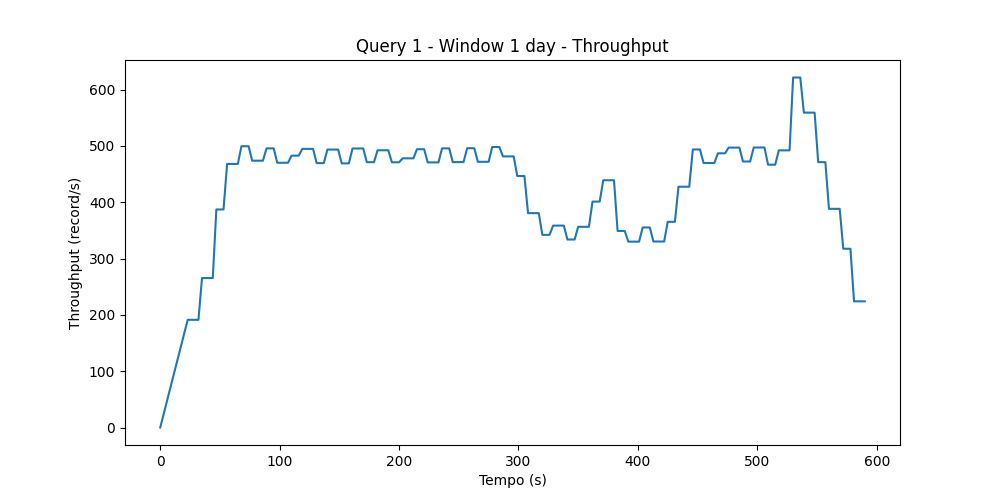
\includegraphics[width=.7\textwidth]{res/q1_w1_throughput.png}
        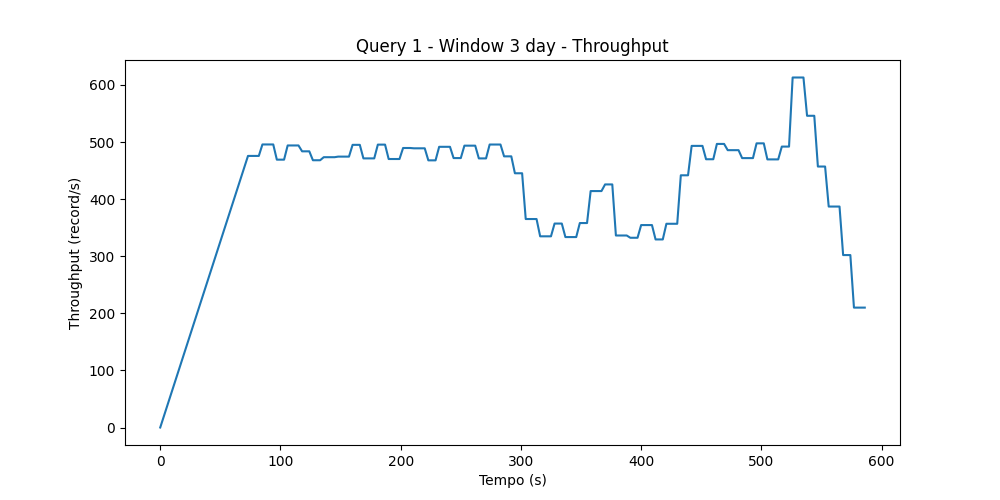
\includegraphics[width=.7\textwidth]{res/q1_w2_throughput.png}
        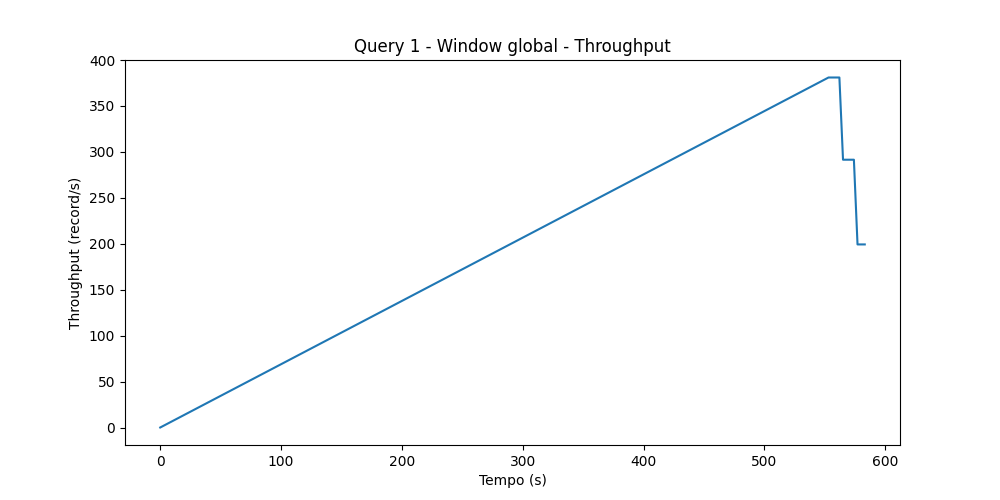
\includegraphics[width=.7\textwidth]{res/q1_w3_throughput.png}
    \end{columns}
\end{frame}


\begin{frame}
    \frametitle{Query2}
    \begin{columns}
        \column{0.5\textwidth}
        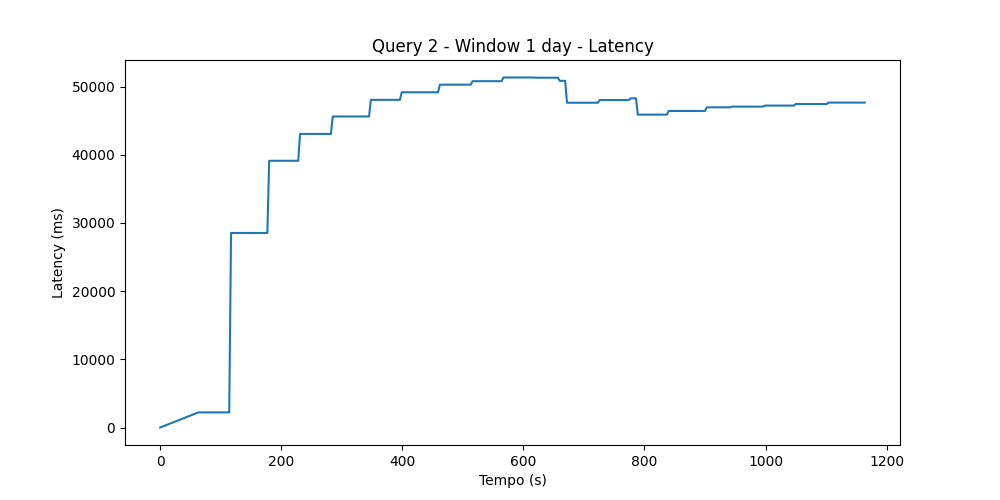
\includegraphics[width=.7\textwidth]{res/q2_w1_latency.png}
        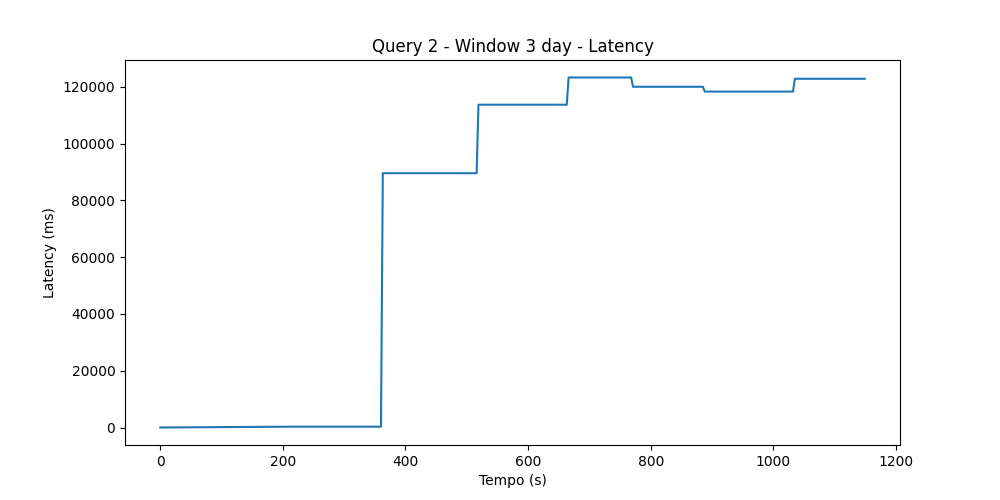
\includegraphics[width=.7\textwidth]{res/q2_w2_latency.png}
        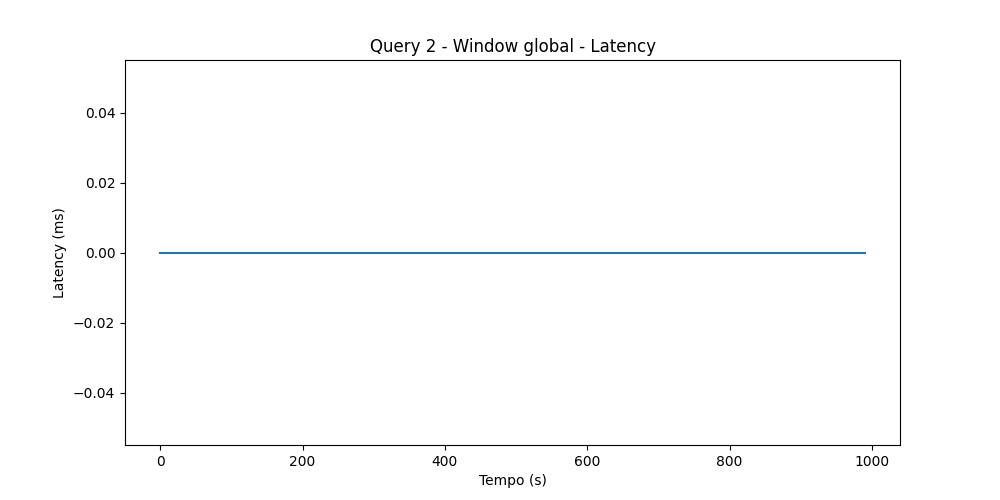
\includegraphics[width=.7\textwidth]{res/q2_w3_latency.png}
        \column{0.5\textwidth}
        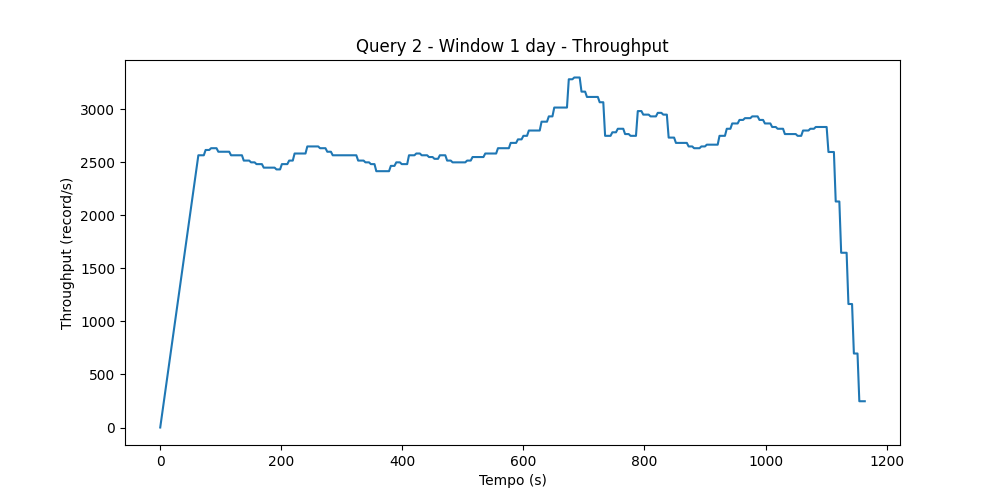
\includegraphics[width=.7\textwidth]{res/q2_w1_throughput.png}
        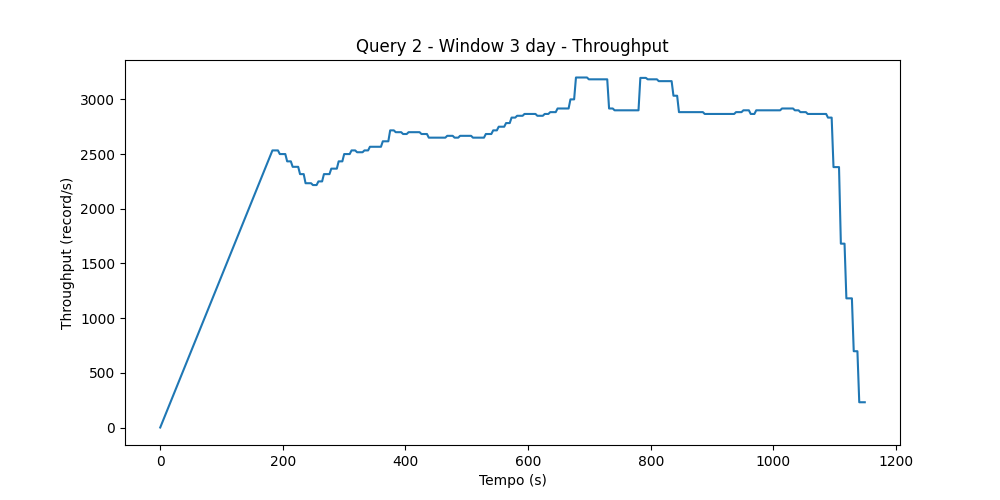
\includegraphics[width=.7\textwidth]{res/q2_w2_throughput.png}
        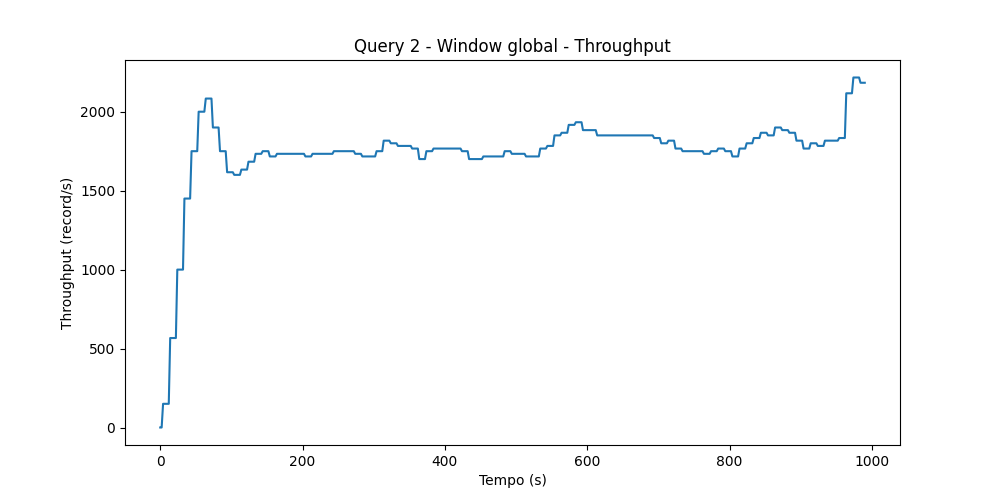
\includegraphics[width=.7\textwidth]{res/q2_w3_throughput.png}
    \end{columns}
\end{frame}


\begin{frame}
    \frametitle{Query3}
    \begin{columns}
        \column{0.5\textwidth}
        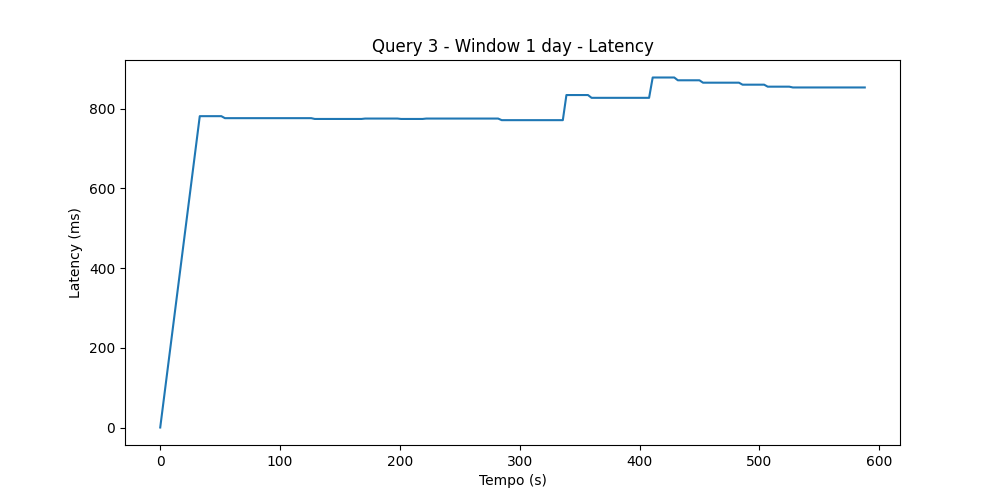
\includegraphics[width=.7\textwidth]{res/q3_w1_latency.png}
        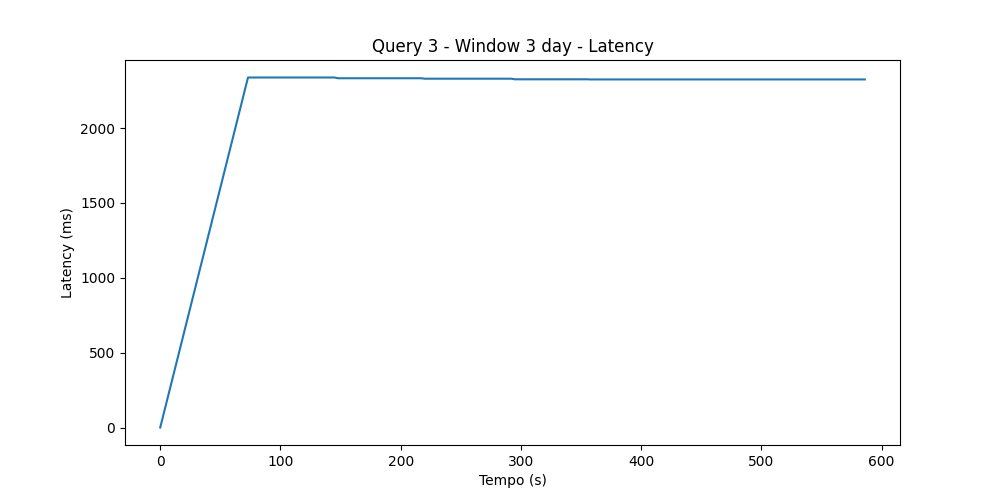
\includegraphics[width=.7\textwidth]{res/q3_w2_latency.png}
        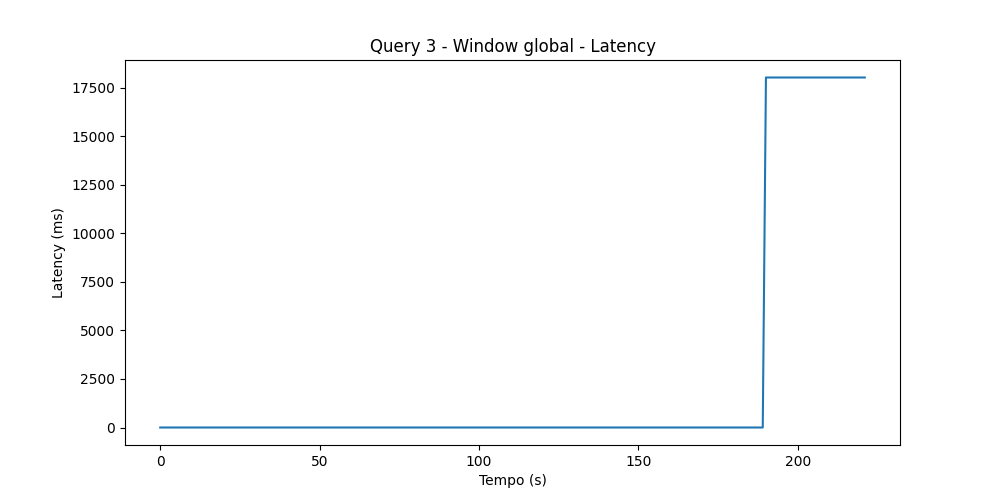
\includegraphics[width=.7\textwidth]{res/q3_w3_latency.png}
        \column{0.5\textwidth}
        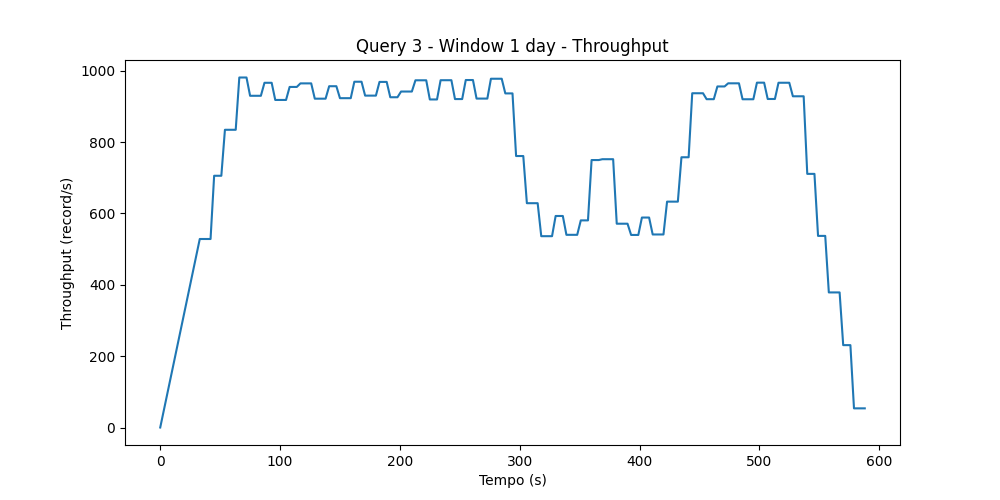
\includegraphics[width=.7\textwidth]{res/q3_w1_throughput.png}
        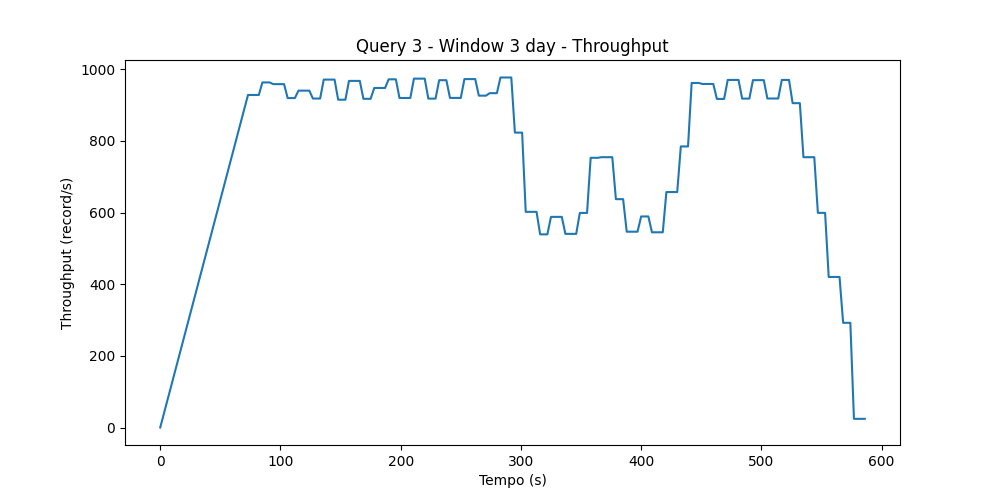
\includegraphics[width=.7\textwidth]{res/q3_w2_throughput.png}
        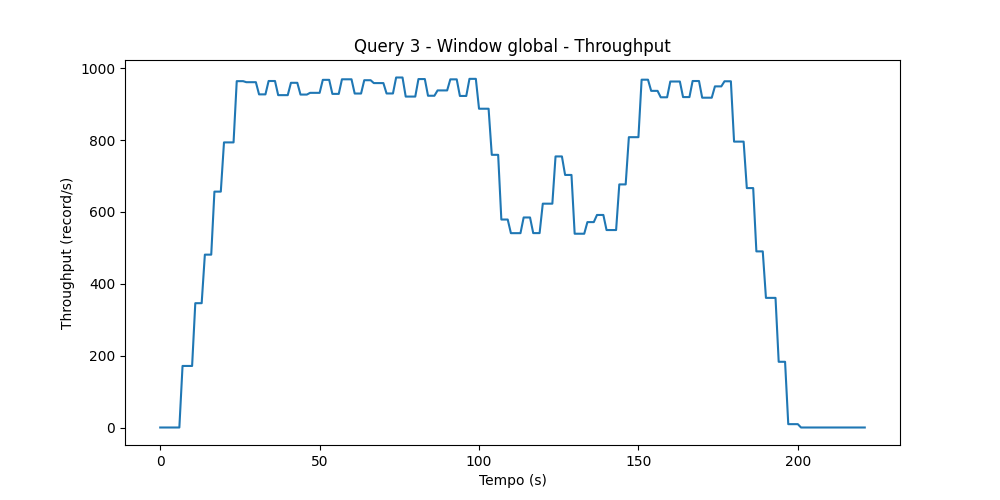
\includegraphics[width=.7\textwidth]{res/q3_w3_throughput.png}
    \end{columns}
\end{frame}


%---------------------------------------------------------
\setLayout{mainpoint}
\begin{frame}{}
    \frametitle{Grazie per l'attenzione}
\end{frame}
%---------------------------------------------------------
\end{document}